\section{Solución propuesta}
\label{sec:Solucion}

Utilizamos la Programación orientada a Aspectos para desarrollar dos
conceptos independientes, {\bf Observable} y  {\bf Transaccional}.

En las secciones subsiguientes se describe el comportamiento de los aspectos, y
en la sección \ref{sec:Union} la integración de ambos aspectos.

\subsection{Aspecto Observable}
	El aspecto Observable convierte los objetos de dominio en objetos observables,
	de una manera transparente y automática, es decir, disparan eventos cada vez
	que el valor de un atributo cambia.

\subsection{Aspecto Transaccional}
	El aspecto Transaccional convierte los objetos en objetos
	transaccionales, en forma transparente  y manteniendo su identidad.
	
	Permite tener un control en las operaciones de modificación de los objetos.
	Permite confirmar la operación, donde sus cambios se impactan en el objeto.
	También permite la cancelación de las operaciones, desechando cada
	modificación realizada. Además soporta el trabajo concurrente, o nivel de
	aislamiento, permitiendo a varios procesos realizar cambios en un mismo objeto
	al mismo tiempo. También soporta múltiples transacciones, ó transacciones
	anidadas.
	
	\bigskip
	
	Interfaz que nos provee las transacciones:
	
	\begin{itemize}
	  \item {\bf \emph{beginTransaction}}  \emph{empezar una transacción}
	  \item {\bf \emph{commit}} \emph{impactar los cambios realizados en esa
	  transacción}
	  \item {\bf \emph{rollback}} \emph{revertir los cambios realizados en esa
	  transacción}
	\end{itemize}


	{\bf Titulo????????}
	\begin{itemize}
	  \item Todo el trabajo se realiza dentro de un contexto transaccional.
	  
	  \item Las modificaciones de los objetos solo pueden ser vistos dento del
	  mismo contexto, si todavía no se hizo el commit.
	   
	  \item El objeto no se modifica, hasta que no se confirme la transacción.
	  
	   \item El contexto transaccional esta asociado a thread actual.
	\end{itemize}

	{\bf Caso de uso}
	
	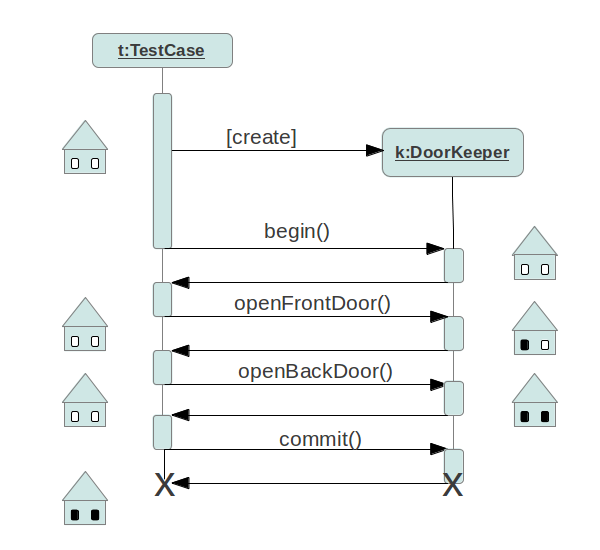
\includegraphics[width=400px, height=300px]{img/tescasePOT}
	
\subsection{Unión de los Aspectos:}
\label{sec:Union}
La unión de los dos aspectos independientes es con el fin de asociar asociar los
eventos disparados por el dominio, con la translación actual.
 
